\documentclass[a4paper,11pt]{article}
\usepackage{amsmath,amsthm,amsfonts,amssymb,amscd,amstext,vmargin,graphics,graphicx,tabularx,multicol} \usepackage[french]{babel}
\usepackage[utf8]{inputenc}  
\usepackage[T1]{fontenc} 
\usepackage[T1]{fontenc}
\usepackage{amsmath,amssymb}
\usepackage{pstricks-add,tikz,tkz-tab,variations}
\usepackage[autolanguage,np]{numprint} 
\usepackage{enumitem}

\setmarginsrb{1.5cm}{0.5cm}{1cm}{0.5cm}{0cm}{0cm}{0cm}{0cm} %Gauche, haut, droite, haut
\newcounter{numexo}
\newcommand{\exo}[1]{\stepcounter{numexo}\noindent{\bf Exercice~\thenumexo} : \marginpar{\hfill /#1}}
\reversemarginpar


\newcounter{enumtabi}
\newcounter{enumtaba}
\newcommand{\q}{\stepcounter{enumtabi} \theenumtabi.  }
\newcommand{\qa}{\stepcounter{enumtaba} (\alph{enumtaba}) }
\newcommand{\initq}{\setcounter{enumtabi}{0}}
\newcommand{\initqa}{\setcounter{enumtaba}{0}}

\newcommand{\be}{\begin{enumerate}}
\newcommand{\ee}{\end{enumerate}}
\newcommand{\bi}{\begin{itemize}}
\newcommand{\ei}{\end{itemize}}
\newcommand{\bp}{\begin{pspicture*}}
\newcommand{\ep}{\end{pspicture*}}
\newcommand{\bt}{\begin{tabular}}
\newcommand{\et}{\end{tabular}}
\renewcommand{\tabularxcolumn}[1]{>{\centering}m{#1}} %(colonne m{} centrée, au lieu de p par défault) 
\newcommand{\tnl}{\tabularnewline}

\newcommand{\trait}{\noindent \rule{\linewidth}{0.2mm}}
\newcommand{\hs}[1]{\hspace{#1}}
\newcommand{\vs}[1]{\vspace{#1}}

\newcommand{\N}{\mathbb{N}}
\newcommand{\Z}{\mathbb{Z}}
\newcommand{\R}{\mathbb{R}}
\newcommand{\C}{\mathbb{C}}
\newcommand{\Dcal}{\mathcal{D}}
\newcommand{\Ccal}{\mathcal{C}}
\newcommand{\mc}{\mathcal}

\newcommand{\vect}[1]{\overrightarrow{#1}}
\newcommand{\ds}{\displaystyle}
\newcommand{\eq}{\quad \Leftrightarrow \quad}
\newcommand{\vecti}{\vec{\imath}}
\newcommand{\vectj}{\vec{\jmath}}
\newcommand{\Oij}{(O;\vec{\imath}, \vec{\jmath})}
\newcommand{\OIJ}{(O;I,J)}

\newcommand{\bmul}[1]{\begin{multicols}{#1}}
\newcommand{\emul}{\end{multicols}}


\newcommand{\reponse}[1][1]{%
\multido{}{#1}{\makebox[\linewidth]{\rule[0pt]{0pt}{20pt}\dotfill}
}}

\newcommand{\titre}[5] 
% #1: titre #2: haut gauche #3: bas gauche #4: haut droite #5: bas droite
{
\noindent #2 \hfill #4 \\
#3 \hfill #5

\vspace{-1.6cm}

\begin{center}\rule{6cm}{0.5mm}\end{center}
\vspace{0.2cm}
\begin{center}{\large{\textbf{#1}}}\end{center}
\begin{center}\rule{6cm}{0.5mm}\end{center}
}



\begin{document}
\pagestyle{empty}
\titre{Programme mon premier jeu sur Scratch}{}{}{}{5eme}

\textbf{{\large Écrire un programme avec Scratch.}}\\

Un programme est constitué de scripts, qui dirigent le comportement d'objets graphiques (appelés « lutins » dans
Scratch), qui peuvent se déplacer, être actifs, ou non. 

Les scripts s'écrivent en emboîtant des « briques » de différentes couleurs.

Pour écrire un script, il suffit de faire glisser les briques depuis la zone des briques vers la zone des scripts. 

Les briques s'emboîtent alors comme dans un puzzle, pour créer des instructions.\\


{\large \textbf{Mon premier jeu}}\\

Programmer un jeu de type « Pacman ».

\bi
\item décor : un labyrinthe
\item personnage 1 : un gentil chat, que le joueur déplace à l'écran à l'aide des touches de direction du clavier.
\item personnage 2 : un fantôme qui se déplace tout seul à l'écran de manière aléatoire.
\item accessoires : des éléments de nourriture.
\ei
Le gentil chat gagne des points en « avalant » la nourriture, et en perd quand le fantôme le touche.\\

\medskip

\begin{flushleft}
\includegraphics[scale=1.3]{jeu1.eps} 
\end{flushleft}

\newpage

\textbf{{\large \begin{center}
Activité 1 – Un personnage à déplacer avec le clavier : le chat
\end{center}}}

Tu vas créer un personnage qui se déplacera à l'écran. Tu pourras le déplacer dans les 4 directions (droite, gauche,
haut, bas) à l'aide des flèches du clavier de l'ordinateur.\\

\underline{Étape 1 }: faire aller le chat vers la droite\\

\noindent 1. L'onglet « Script » est sélectionné.\\
2. Clique sur le bouton « Evènements » (bord marron).\\
3. Fais glisser la brique marron « quand espace est cliqué » vers la zone de script.\\
4. Clique sur la petite flèche à côté de « espace » et choisis « flèche droite »\\
5. Clique sur le bouton « Mouvement » (bord bleu), et fais glisser la brique bleue « s'orienter à 90 » vers la zone de script.\\
6. Emboîte la brique « s'orienter à 90 » et la brique « quand flèche droite est pressée ».\\
7. Fais glisser la brique bleue « avancer de 10 pas » vers la zone de script.\\
8. Emboîte la brique « avancer de 10 pas » avec la brique « s'orienter à 90 ».\\
9. Appuie sur la flèche droite du clavier, et regarde le personnage aller vers la droite.\\

\underline{Étape 2} : faire aller le chat vers la gauche\\

\noindent 10. Clique sur le bouton « Evènements » (bord marron).\\
11. Fais glisser la brique marron « quand espace est cliqué » vers la zone de script.\\
12. Clique sur la petite flèche à côté de « espace » et choisis « flèche gauche »\\
13. Clique sur le bouton « Mouvement » (bord bleu), et fais glisser la brique bleue « s'orienter à 90 » vers la zone de script.\\
14. Clique sur la petite flèche noire située à droite de 90, et sélectionne -90.\\
15. Emboîte la brique « s'orienter à -90 » et la brique « quand flèche gauche est pressée ».\\
16. Fais glisser la brique bleue « avancer de 10 pas » vers la zone de script.\\
17. Emboîte la brique « avancer de 10 pas » avec la brique « s'orienter à -90 ».\\
18. Appuie sur la flèche gauche du clavier, et regarde le chat aller vers la gauche.\\
19. Problème : il a la tête en bas. Pour y remédier affiche le menu contextuel du chat, avec le bouton droit de
la souris, et sélectionne « info » (Repère 1) . Choisis le style de rotation 
\includegraphics[scale=1]{fleche.eps} ,  retournement gauche/droite uniquement.\\

\includegraphics[scale=1.2]{jeu2.eps} \\

\underline{Étape 3} : Faire aller ton lutin dans les quatre directions\\

\noindent 20. Complète ton script pour que le chat puisse être déplacé vers le haut et vers le bas, avec les flèches haut et bas du clavier.\\
Essaye !\\
21. N'oublie pas de sauvegarder ton programme en l'enregistrant dans ton espace de travail sur le serveur du collège.
(Fichier - Enregistrer sous - ordinateur - ...)\\


\textbf{{\large \begin{center}
Activité 2 – « Sentir » le monde et utiliser des instructions conditionnelles\\
\end{center}}}

\underline{Étape 1} : dessiner un labyrinthe\\

\noindent 1. Clique sur l'outil « Dessiner un nouveau lutin ». Cet outil a la forme d'un pinceau (Repère 2 page 2).\\
Utilise l'outil Zoom(-) pour voir toute la zone de dessin.\\
2. Dessine les murs, le plus simple est d'utiliser l'outil ligne. Attention à bien laisser des zones transparentes (damier gris et blanc), ces zones seront les zones de déplacement du chat.\\
3. Clique sur l'onglet script pour revenir à l'écran de travail.\\
4. Renomme les lutins, « le chat » et « labyrinthe », par la commande « info » (Repère 1 page 2) Il sera peut-être nécessaire de redimensionner le chat avec les outils « Agrandir » et « Réduire » (repère 4 page 2)\\

\underline {Étape 2} : rebondir sur les murs\\

\noindent 5. Dans la zone de script du chat, ajoute les briques ci-contre.\\

\bmul{2}
Pour rebondir sur les murs du labyrinthe
Attention : si la valeur 10 est trop faible, dans ce cas le chat « traversera » les murs, il faudra alors choisir une valeur plus grande.\\

Pour que le chat rebondisse sur le bord de l'écran.\\

\columnbreak


\includegraphics[scale=1.2]{jeu3.eps} 

\emul

6. N'oublie pas de sauvegarder ton programme en l'enregistrant dans ton espace de travail sur le serveur du collège.
(Fichier - Enregistrer sous - ordinateur - ...)\\

\textbf{{\large \begin{center}
Activité 3 – Quelque chose à manger. Conditions, variables, (in)visibilité\\
\end{center}}}

\underline{Étape 1 }: créer de la nourriture\\

\noindent 1. Clique sur l'outil « choisir un lutin dans la bibliothèque ». Cet outil a la forme d'un visage de lutin (Repère 3 page 2).\\
2. Valide par un double-clic un objet qui représentera la nourriture, et réduit sa taille autant que nécessaire
avec les outils redimensionner (Repère 4 page 2)\\
3. Renomme l'objet, dans cet exemple il est nommé banane.\\

\underline{Étape 2} : créer un script pour afficher le score et rendre la nourriture mangée invisible\\

\noindent 4. Clique sur le bouton « données » (bord orange, puis sur « Créer une variable », pour tous les lutins.
Nomme cette variable score.\\

\newpage

\noindent 5. Dans la zone de script de la banane, glisse des briques permettant :\\
- l'affichage du score\\
- la « disparition » de la nourriture mangée (montrer/cacher)\\
- le comptage du score (1 point de plus à chaque nourriture mangée)\\
- la remise à 0 du score au démarrage d'une nouvelle partie.\\

\noindent 6. N'oublie pas de sauvegarder ton programme en l'enregistrant dans ton espace de travail sur le serveur du collège.
(Fichier - Enregistrer sous - ordinateur - ...)\\

\includegraphics[scale=1.25]{jeu4.eps} \\


\underline{Étape 3} : dupliquer la nourriture\\

\noindent 7. Une fois que tu es satisfait de ton objet « nourriture » et de son script, tu peux le dupliquer en utilisant l'outli « tampon ».\\
Clique sur l'outil « tampon » en haut de l'écran (repère 5 page 2), et clique ensuite sur l'objet que tu souhaites dupliquer,et ceci autant de fois que nécessaire. Tu remarqueras que l'objet est copié avec son script !\\
8. Dispose la nourriture dans tout le labyrinthe.\\
9. Teste le résultat et n'oublie pas de sauvegarder.\\


\textbf{{\large \begin{center}Activité 4 – Un fantôme à éviter.
Opérateurs, nombre aléatoire.
\end{center}}}

\underline{ Étape 1} : créer un fantôme qui rebondit de manière aléatoire\\

\noindent 1. Choisis un nouveau lutin que tu vas nommer fantôme.

\noindent 2. Programme-le pour qu'il se déplace tout seul, et qu'il
rebondisse sur les bords de l'écran avec une direction aléatoire.\\
Voici un exemple de script ci-contre, tu peux en trouver d'autres, modifier les valeurs..\\



\begin{center}
\includegraphics[scale=1]{jeu5.eps} 
\end{center}

\newpage
\underline{Étape 2} : un contact entre le fantôme et le chat
fait baisser le score.\\

Ci-dessous une possibilité de script, il est possible
qu'il ne convienne pas à ton jeu. Modifie alors
les valeurs numériques, les instructions…\\


\begin{center}
\includegraphics[scale=1]{jeu6.eps} 
\end{center}


Teste ton jeu et n'oublie pas de sauvegarder !

\begin{center}
 
\includegraphics[scale=1.2]{jeu7.eps}
 \end{center} 

\end{document}
